\begin{savequote}[75mm] 
Nulla facilisi. In vel sem. Morbi id urna in diam dignissim feugiat. Proin molestie tortor eu velit. Aliquam erat volutpat. Nullam ultrices, diam tempus vulputate egestas, eros pede varius leo.
\qauthor{Quoteauthor Lastname} 
\end{savequote}

\chapter{The title of chapter one}

- radiotherapia oggi (vs surgery and chemio) - serve fonte

- serve fonte, ho usato katia parodi

Results of radiotherapy are improved when a high dose of radiation with highbiological effectiveness is delivered to the tumor with the least possible dose to the sorrounding tissues, especially in the case of critical organs.
In order to increase the conformity of the dose delivered to the tumor, diverse technologies have been considered and used.
Traditional forms of radiotherapy, X-ray tubes (energy $\sim$ 100 keV) or radioactive isotopes have been replaced by linear accelerators delivering $\sim$ 10 MeV from different directions (e.g. Intensity Modulated Radio Therapy), and provide treatment with photons and electrons.
Though being widely used as a standard in radiation therapy, the effectiveness of conventional electromagnetic radiation is limited by the intrinsic characteristics of interaction with matter.
In particular two aspects unfavours in principle the usability of electromagnetic radiation with respect to ion for tumor targeting: the depth dose profile, which does not allow for an optimal dose deposition to the tumor sparing vital organs
and the inferior biological efeffectiveness, which is the limiting factor in case of radioresistant tumors.
Heavier charged particles, like protons and ions (He-Ca) have the potentiality to overcome the limits of convetional therapy With respect to this, the scientific community is directing his attention towards possible improvements of ion beam therapy.

- qui citare entervision website

The work outlined in these pages have been sponsored by  The European training network in digital medical imaging for radiotherapy (ENTERVISION) at the European Center of Nuclear Research (CERN). ENTERVISION was established in February 2011 in response to the critical need for reinforcing research in online 3D digital imaging and the training of professionals in order to deliver some of the key elements and building blocks for realizing the vision for early detection and more precise treatment of tumours.

\section{Hadrontherapy}
\subsection{Ion beam therapy}

The first proposition of ion beam therapy was presented in 1946 by R. Wilson. The original idea was exploit the physical properties of ion interaction in matter to improve the precision in radiotherapy treatments.  
Making use of the so called Bragg peak, that is using the fact that protons and ions in general deposit a maximum of energy at the end of their trajectory, the treatment could save the sorrounding tissue from radiation overdose.

The dose deposited by photons, considered as the gold standard for tumor treatment, is maximum close to the beginning of the trajectory in the body and is characterized by an exponential decrease. As a consequence an undesired radiation dose is delivered to healthy tissues around the targeted tumor.


\subsection{Beam delivery}

\section{PET - TOFPET}
\subsection{Monitoring of the beam}
\subsection{PET principles}
\subsection{TOFPET}



\section{CERN}
\section{MEDICAL PHYSICS - HIGH ENERGY}


- STUDY OF TIME PROFILES



$x = 1/\alpha$ 

\cite{Eigen1971, Knuth1968}

$$\zeta = \frac{1039}{\pi}$$

Fig.~\ref{fig:myFullPageFigure}.

\begin{figure}  
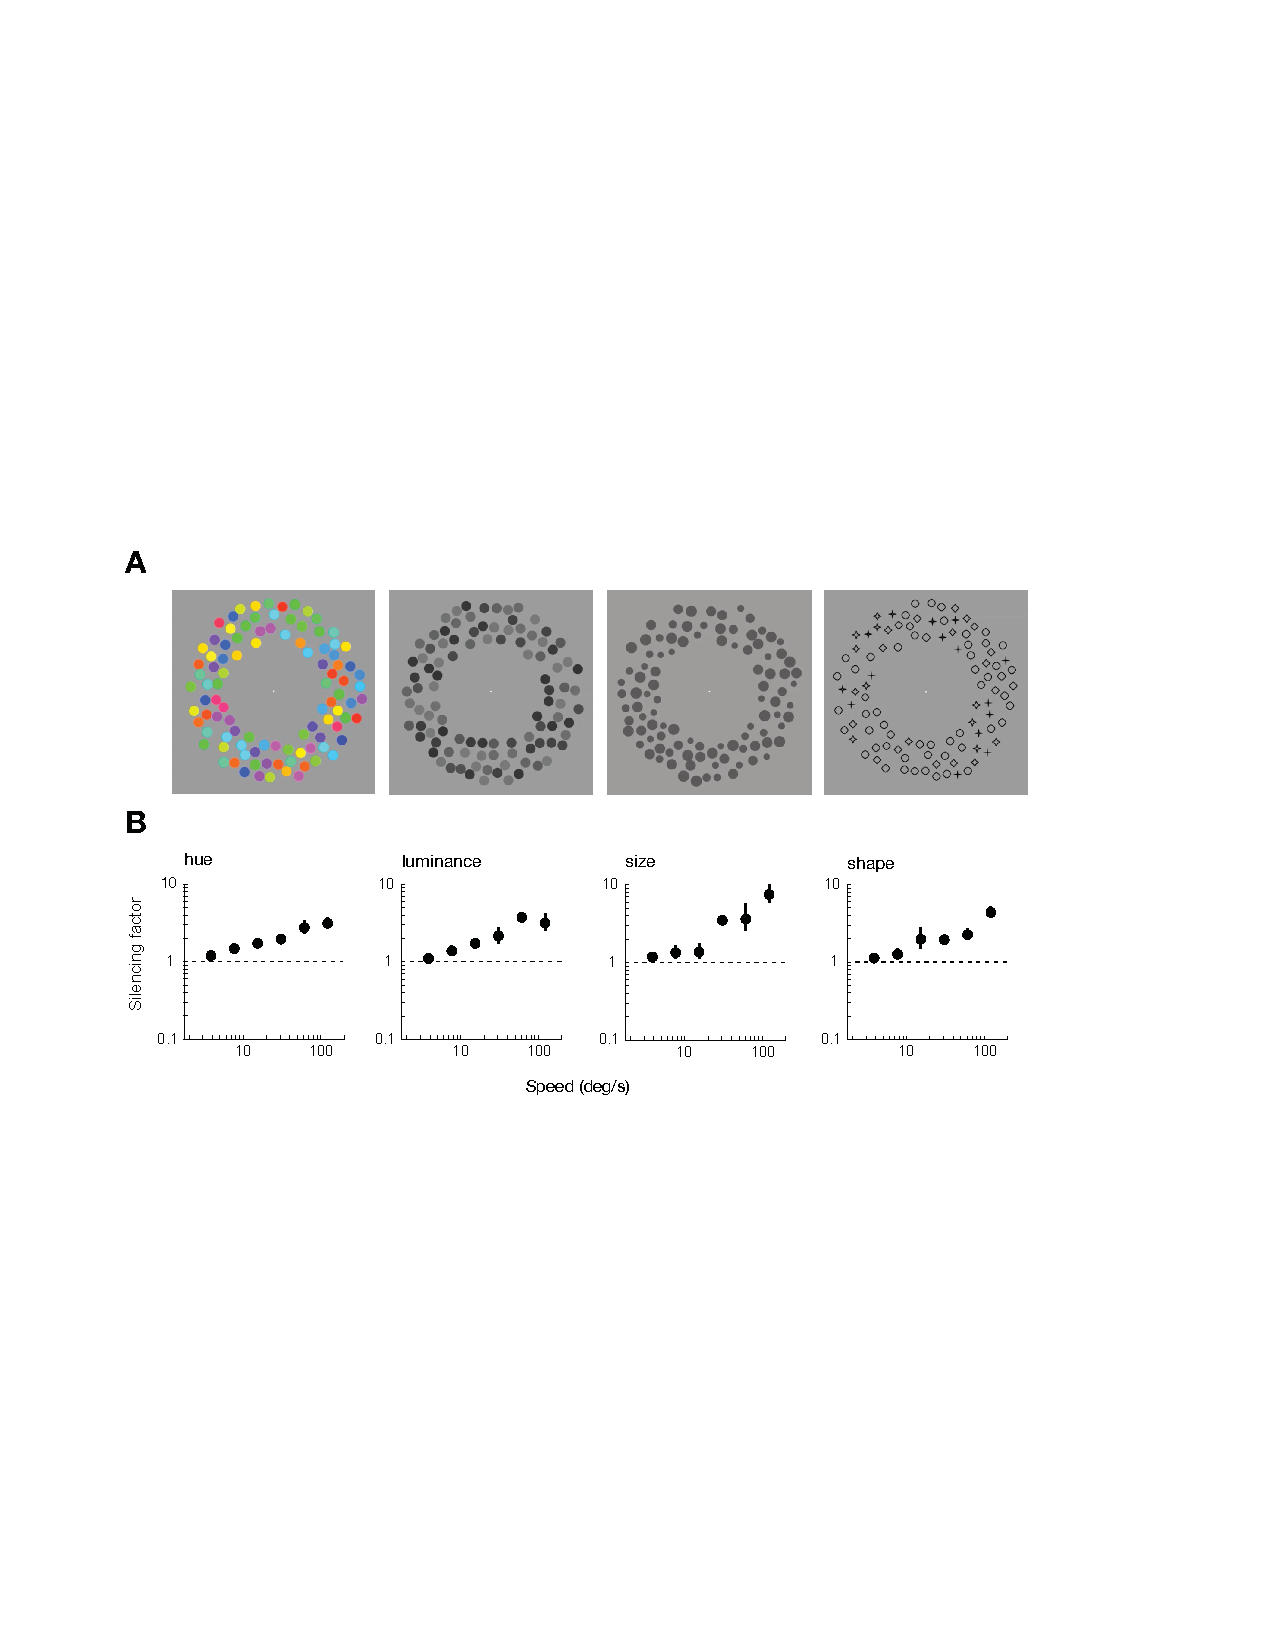
\includegraphics[width=\textwidth]{figures/fig1}
\caption[Short figure name.]{This is a figure that floats inline and here is its caption.
\label{fig:myInlineFigure}}
\end{figure}

\afterpage{\clearpage}


